%%%%%%%%%%%%%%%%%%%%%%%%%%%%%%%%%%%%%%%%%%%%%%%%%%%%%%%%%%%%%%%%%%%%%%%%%%%%%%%%
\chapter{Método Proposto incluído}

O método proposto deve receber como entrada um conjunto de treino, a partir do qual um modelo é construído. Quando uma nova instância é recebida este modelo pode ser usado para gerar uma lista ordenada de saída (ranking). Esta lista é composta pelos valores de classe (do conjunto de treino) mais prováveis para aquela instância, de forma que o primeiro valor é o mais provável. 

O método proposto compreende um meta-classificador que por sua vez é composto por um conjunto de classificadores internos. Estes diversos classificadores são empregados em cascata para gerar a lista ordenada de saída. Note que, cada item da lista é dado por apenas um classificador interno. A Figura \ref{fig:metodoproposto01} ilustra como a lista de saída é gerada pelos classificadores internos.

\begin{figure}[h!]
  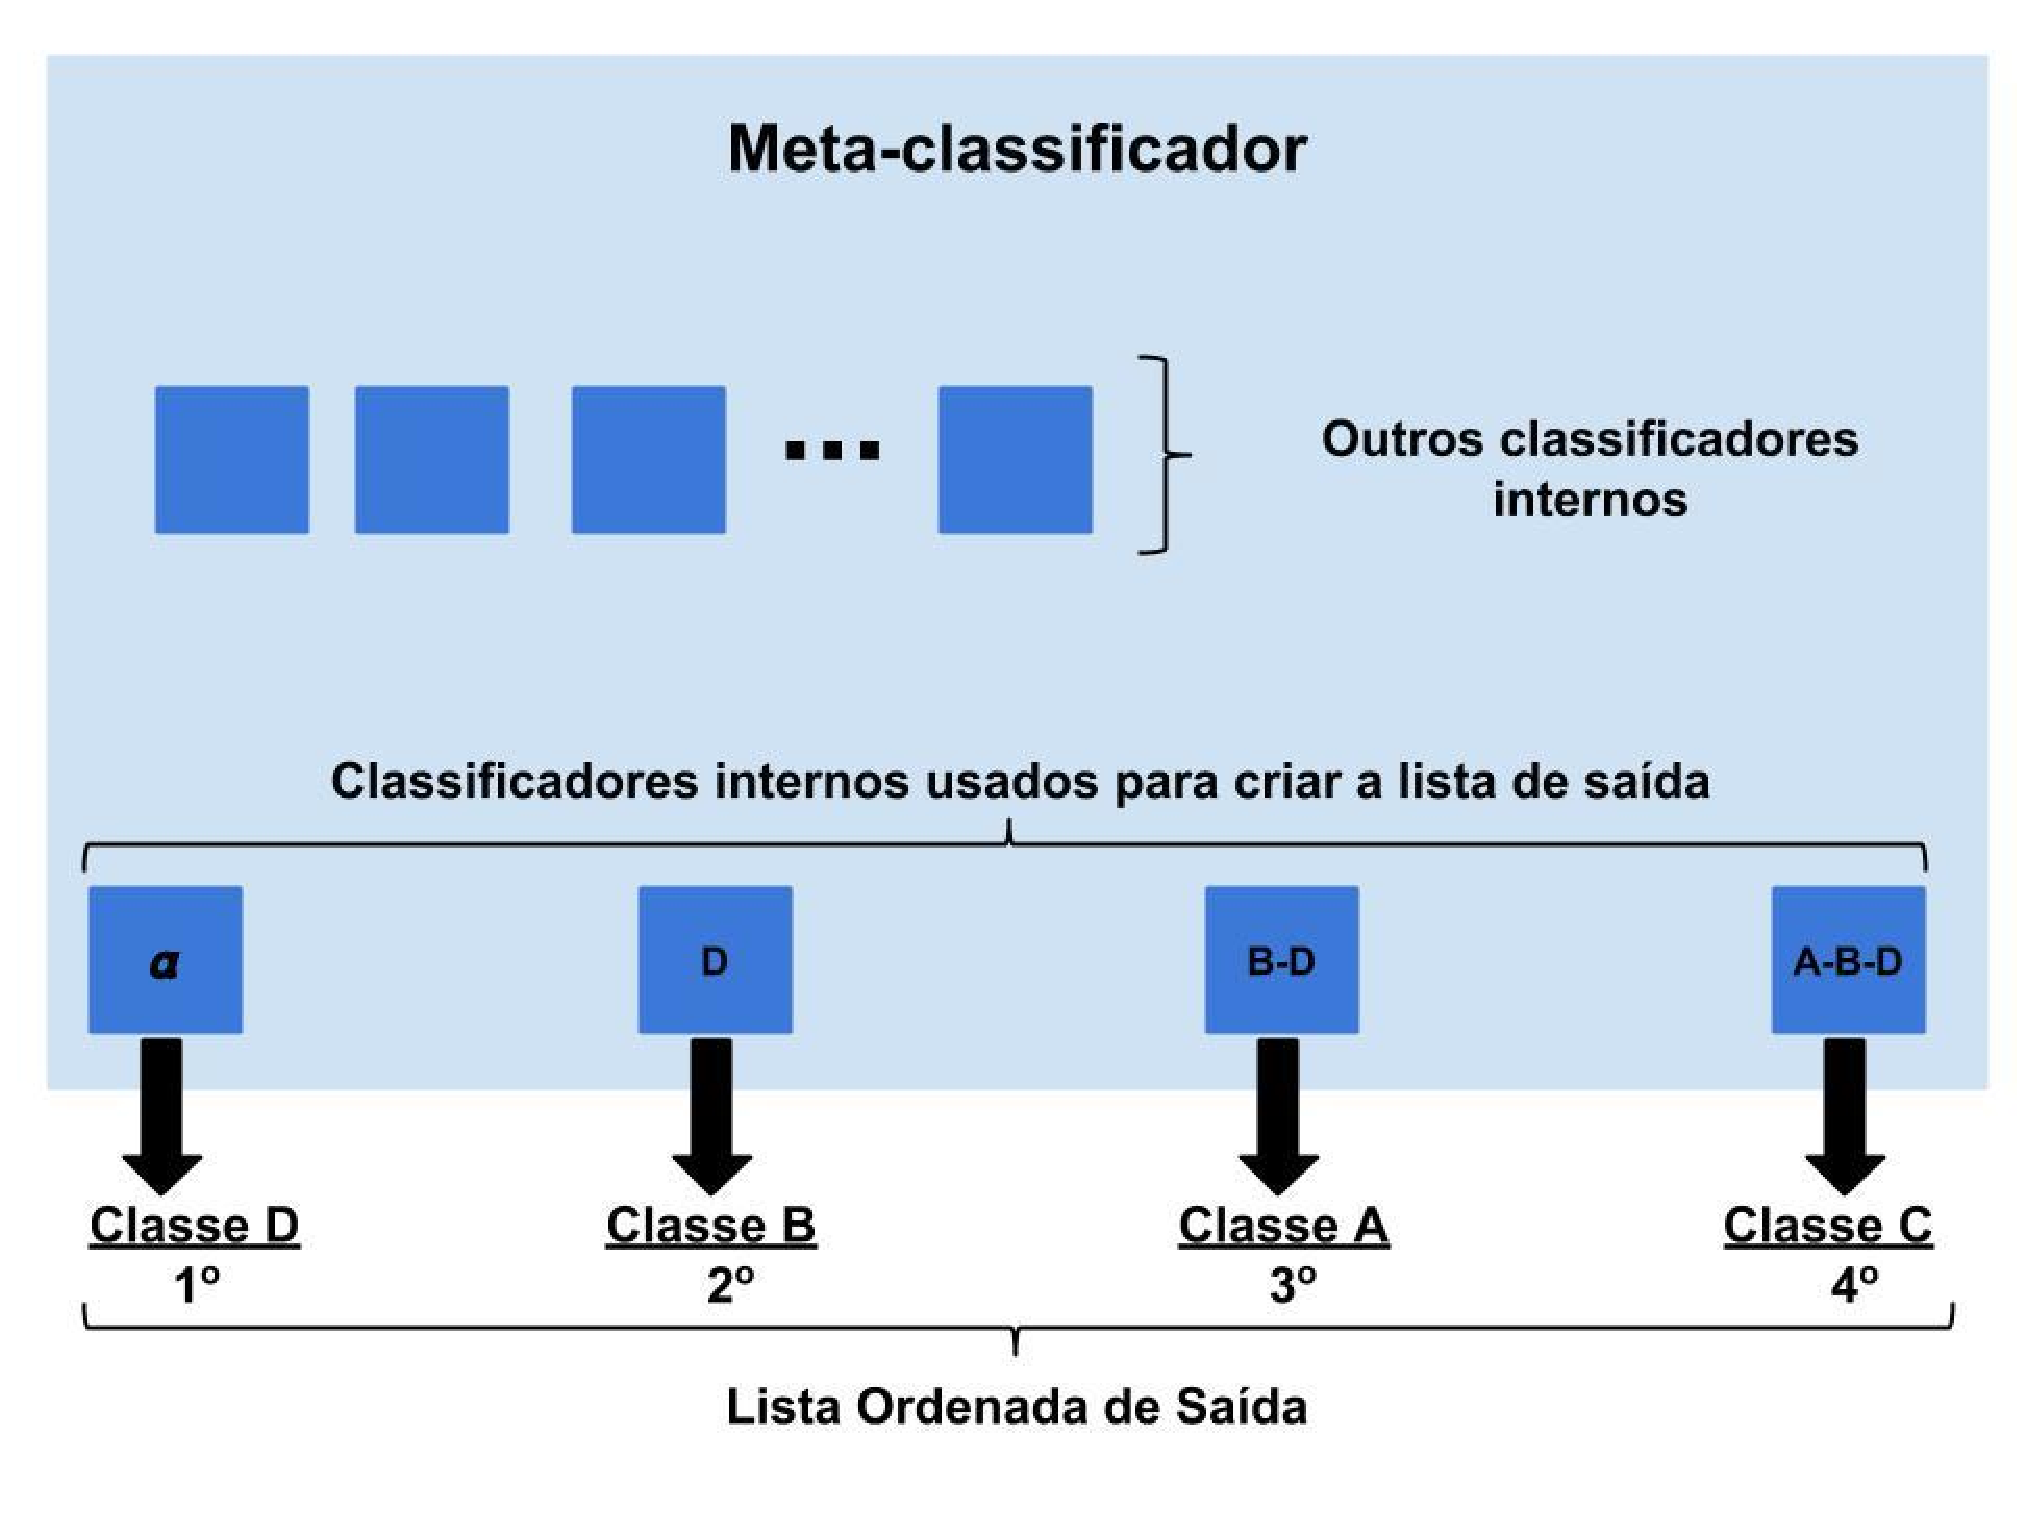
\includegraphics[width=\linewidth]{images/metodoproposto01.eps}
  \caption{Classificadores em cascata e lista de saída.}
  \label{fig:metodoproposto01}
\end{figure}

Assuma que temos 5 classes distintas no conjunto de dados: A, B, C e E. No exemplo da Figura \ref{fig:metodoproposto01} queremos gerar uma lista de saída de tamanho quatro, logo quatro classificadores internos são utilizados. O classificador inicial (alfa) sempre gera o primeiro item de uma lista. O meta-classificador precisa então escolher um de seus classificadores internos para gerar um próximo item. Como a figura sugere, esta escolha depende de todos os elementos inseridos anteriormente. Por exemplo, na figura o classificador B-D foi usado para gerar o terceiro elemento da lista pois as classes B e D já tinham sido colocadas na mesma.

\section{Treinamento do Meta-classificador}

Seja \textit{T} o conjunto de treino do meta-classificador e \textit{v} o número de valores distintos que seu atributo classe pode assumir. Este conjunto será filtrado de formas diferentes e utilizado para treinar os classificadores internos. Somente o classificador inicial, usado para gerar o primeiro elemento da lista de saída, é treinado com o conjunto de treino \textit{T} completo. Qualquer outro classificador interno é treinado com um conjunto de treino filtrado. Em geral, o classificador que será usado para classificar o item da lista na posição \textit{k}, onde \textit{k} $<$ \textit{v}, deve ser treinado com um conjunto de treino filtrado \textit{k-1} vezes. Estas filtragens retiram sucessivamente do conjunto de treino as instâncias cujas classes já foram colocadas na lista. Este processo é ilustrado na Figura \ref{fig:metodoproposto02}.

\begin{figure}[h!]
  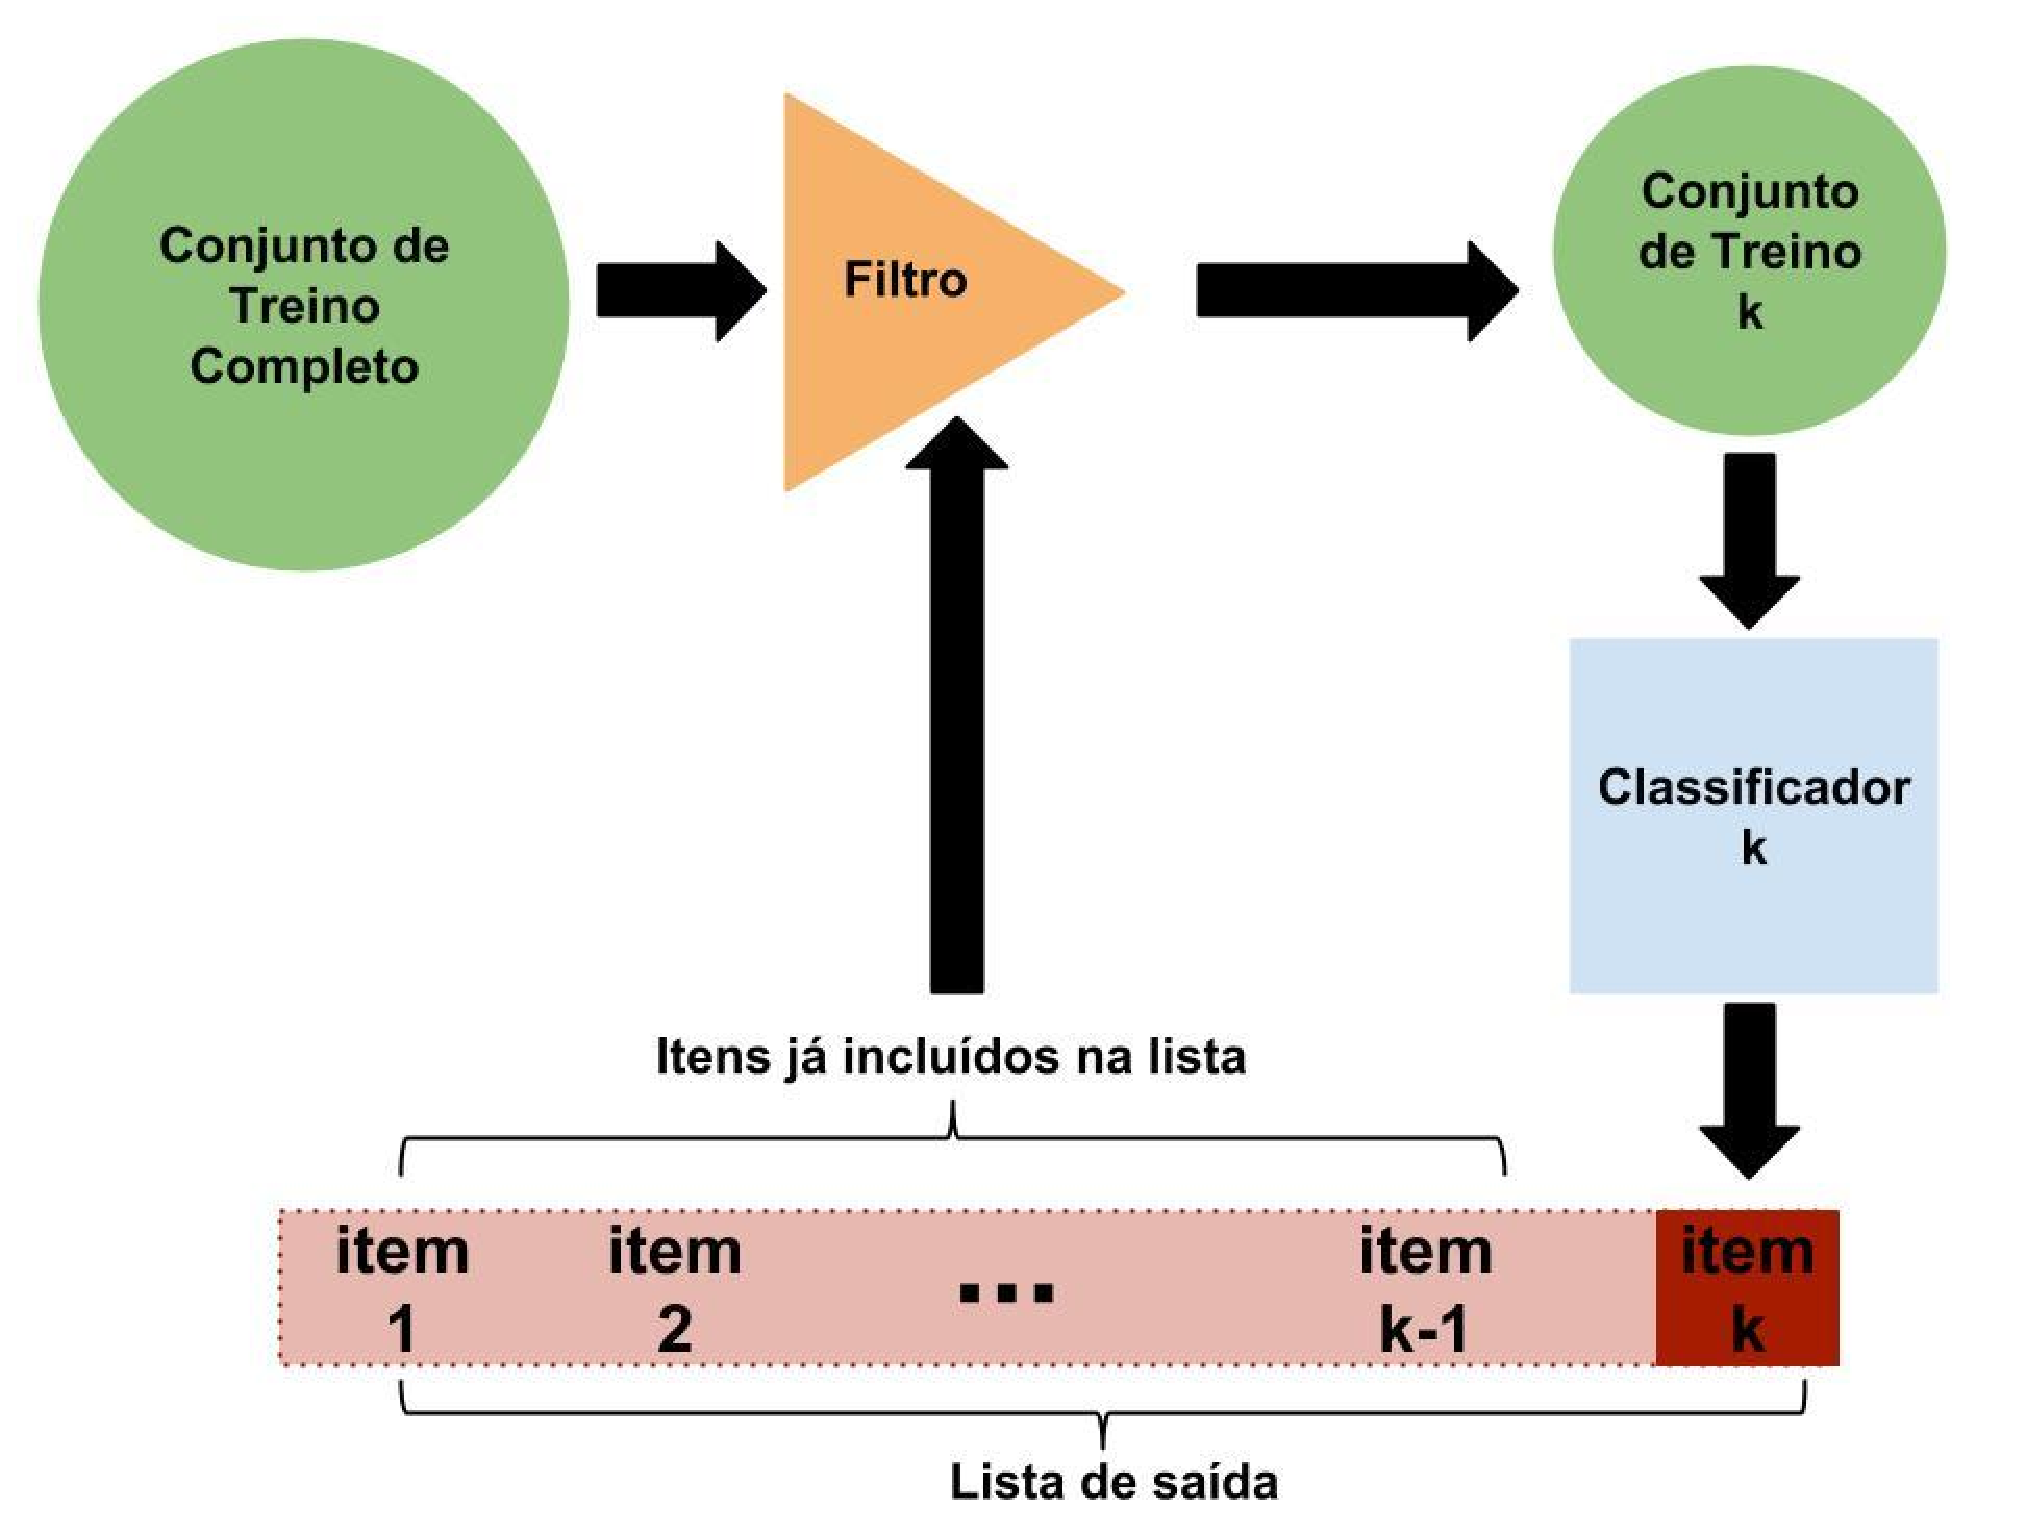
\includegraphics[width=\linewidth]{images/metodoproposto02.eps}
  \caption{Filtragem do conjunto de treino e treinamento de um classificador.}
  \label{fig:metodoproposto02}
\end{figure}


Note que o meta-classificador não foi desenvolvido para receber um conjunto de treino com uma lista ordenada no gabarito. 
Ele deve ser treinado com \textit{datasets} que apresentam apenas um único valor no atributo classe.
Apos o treinamento com um conjunto de dados deste tipo o meta-classificador é capaz de gerar uma lista ordenada de classes para uma nova instância.

\section{Versões do método}

O método proposto foi desenvolvido em duas versões: estático e dinâmico.


\subsection{Método Estático}

O método estático gera a priori todas os subconjuntos de classe que podem compor a lista de saída. Ele então treina todos os possíveis classificadores, cada um com sua versão filtrada do conjunto de treino, armazenando-os internamente. Este conjunto de classificadores internos é efetivamente o modelo gerado pelo meta-classificador. Este pode ser usado então para gerar rankings ao receber novas instâncias. Note que, quanto mais valores a classe do conjunto de treino original puder assumir, mais classificadores internos comporão o modelo do meta-classificador.

Sejam \textit{N} o número de classificadores geados pelo método estático, \textit{v} o número de valores de classe distintos no conjunto universo e \textit{k} o tamanho da lista que se deseja gerar. De forma geral, considerando que $\textit{k} \leq \textit{v}$, temos que:

\begin{equation*}

\textit{N} = \sum\limits_{i=0}^k \binom{v}{i}

\end{equation*}

A Figura \ref{fig:metodoproposto03} ilustra os classificadores internos gerados quando as possibilidades de valor de classe são A, B, C e D. Na figura as numerações não somente identificam cada classificador interno, elas denotam como o conjunto de treino foi filtrado para gerar aquele classificador. Além disso, a figura divide os classificadores internos em camadas. Um classificador que pertence a camada \textit{k} pode ser usado apenas para gerar um elemento na posição \textit{k} da lista de saída.

\begin{figure}[h!]
  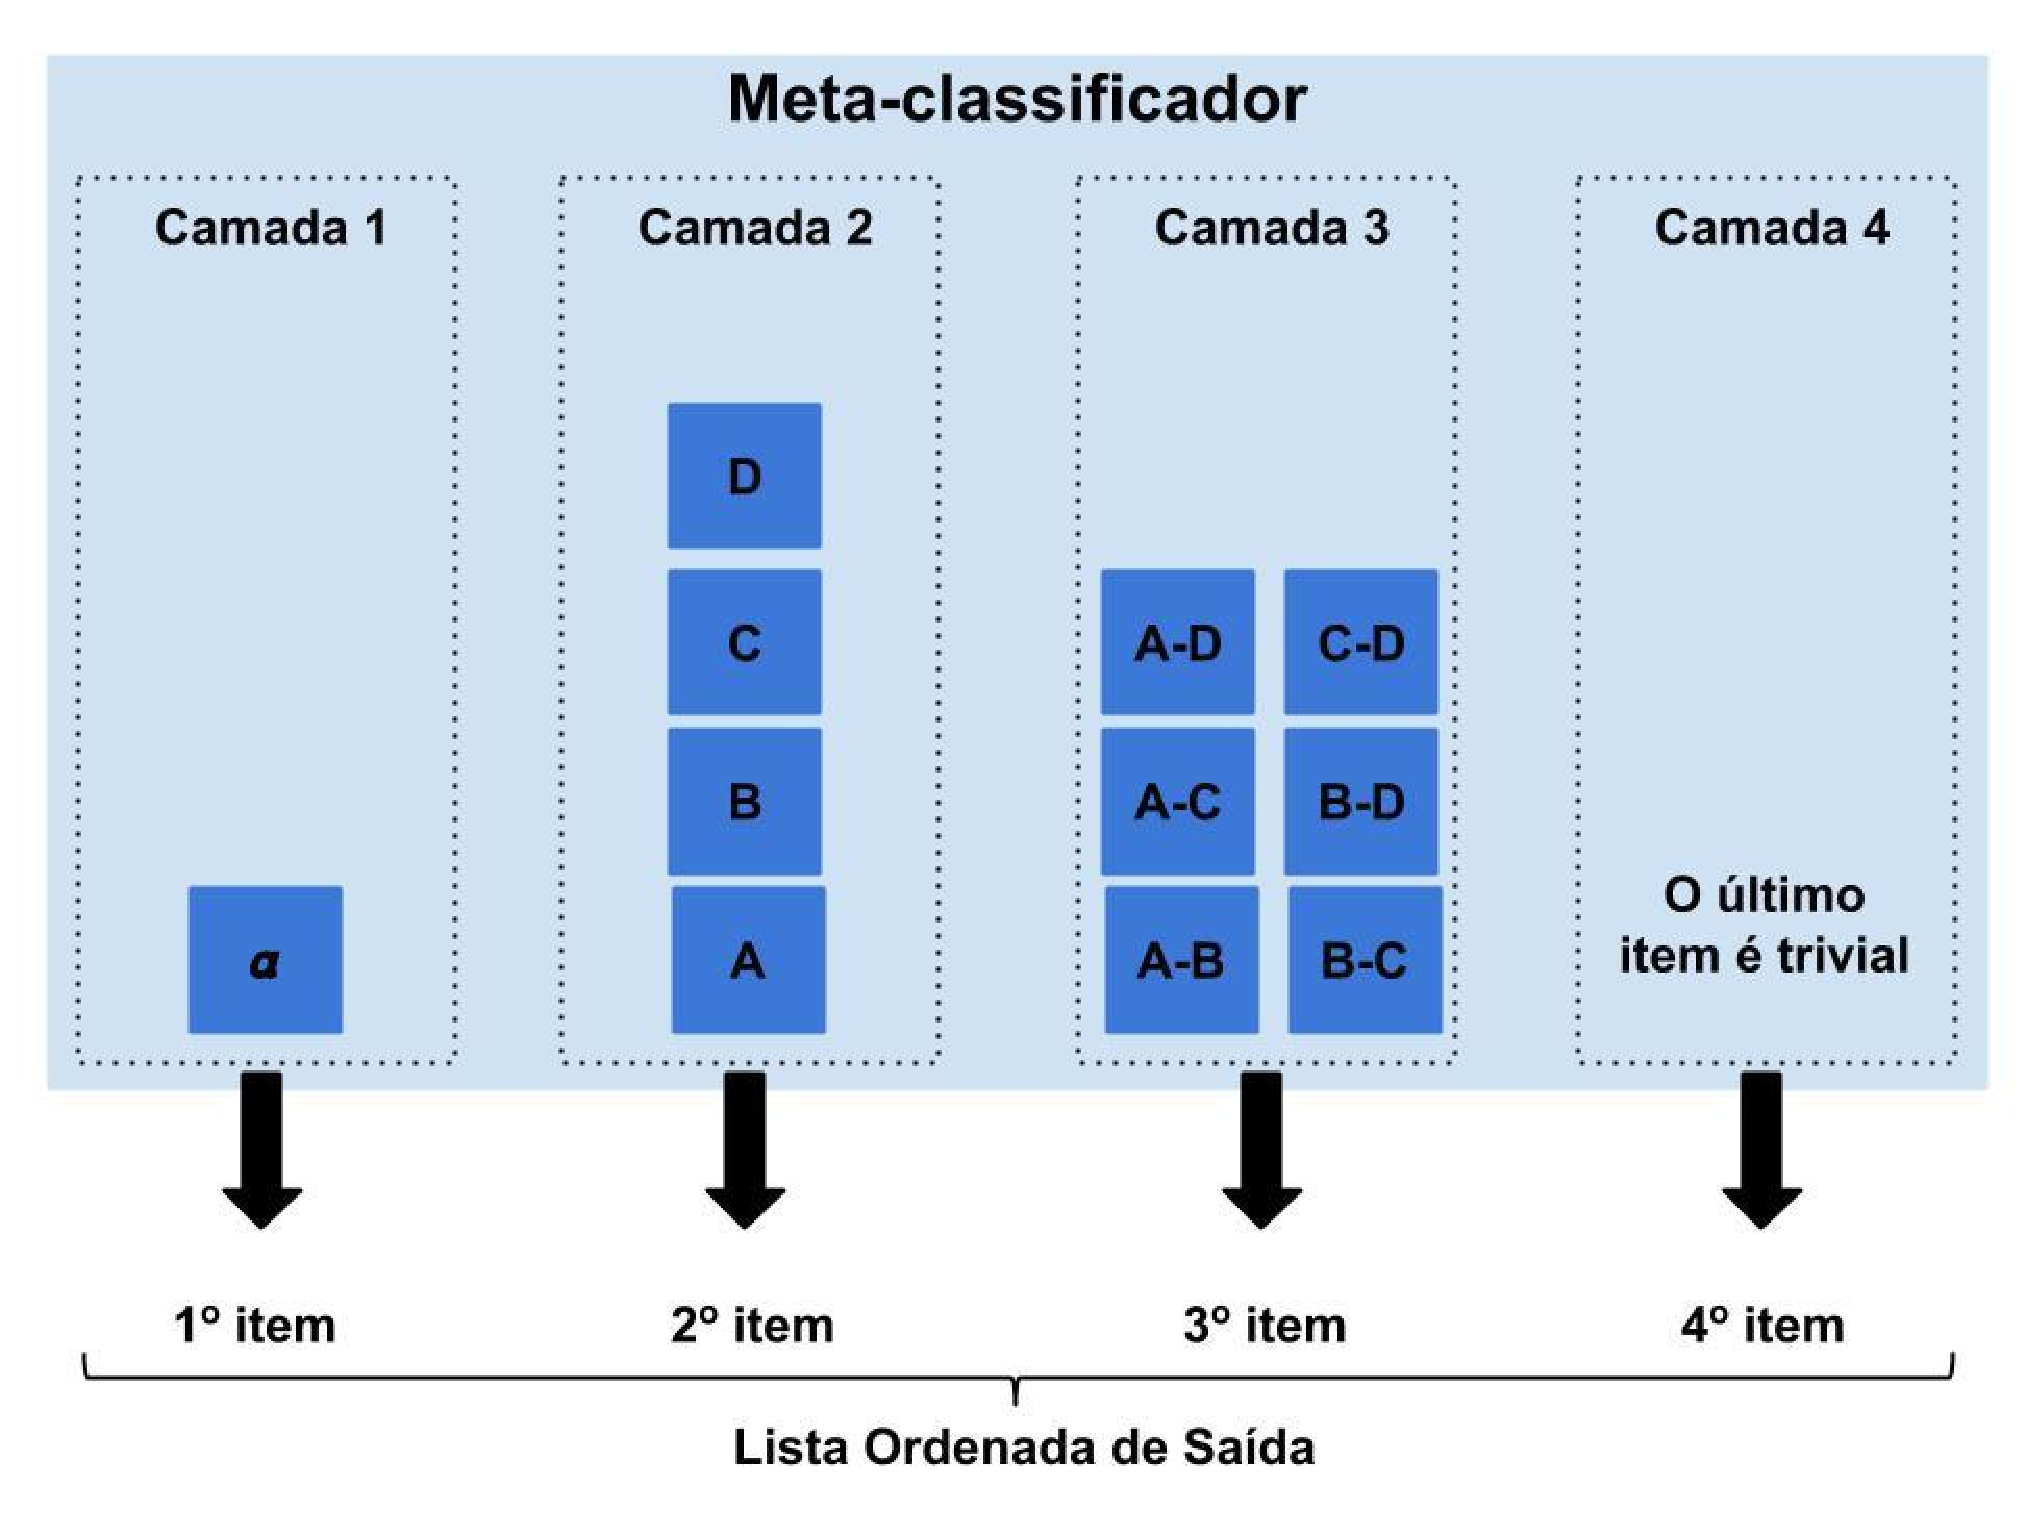
\includegraphics[width=\linewidth]{images/metodoproposto03.eps}
  \caption{Camadas de classificadores intenos.}
  \label{fig:metodoproposto03}
\end{figure}

A versão estática pode ser lenta durante a fase de treinamento, pois precisa treinar um grande número de classificadores antes de classificar qualquer nova instância. Por outro lado, uma vez treinado o modelo pode ser usado para classificar diversas novas instâncias rapidamente.

\subsection{Método Dinâmico}

O método dinâmico constrói o modelo na medida do necessário, treinando apenas os classificadores requeridos para a construção da lista de saída para a instância em questão. Ou seja, o modelo é treinado ao mesmo tempo que a classificação de instâncias é feita. De forma análoga ao método anterior, os classificadores são armazenados internamente a medida que são treinados. Desta forma, ao construir a lista de saída, os classificadores já treinados são reutilizados. Sendo assim, um mesmo classificador nunca é treinado mais de uma vez. 

Esta segunda versão tende a ser mais rápida do que a anterior, visto que não precisa treinar todas as possíveis combinações de classificadores a priori. Entretanto, como o treinamento do modelo é feito ao mesmo tempo que a classificação de instâncias, o tempo de classificação da versão dinâmica é maior do que a versão estática. 

Concretamente, sejam \textit{k} o tamanho da lista de saída, \textit{M} o tempo médio de treinamento de um classificador interno e \textit{t} o tempo médio de classificação de um único ítem por um classificador interno já treinado. Note que tipicamente temos que $ \textit{M} >> \textit{t} $. Considere o caso onde o meta-classificador ainda não tem um classificador interno treinado. Usaremos este como limite superior para o tempo de construção da lista de saída para uma nova instância. Este tempo é calculado por $ \textit{T} = \textit{k}\left(\textit{M} + \textit{t}\rigth) $. Por outro lado, o limite inferior para o tempo \textit{T} ocorre no caso onde o meta-classificador já treinou a priori todos os classificadores internos necessários na construção da lista de saída de uma nova instância. Neste caso temos $ \textit{T} = \textit{k}\textit{t} $.

\section{Vantagens e Desvantagens do método}

O método proposto tem a versatilidade de permitir o uso que qualquer classificador internamente. Além disso, as sucessivas filtragens do conjunto de treino removem as instâncias com classes que não são mais pertinentes para construção da lista de saída. Estas duas carcterísticas podem contribuir para melhoria do resultado final com (1) a escolha do classificador interno mais adequado e (2) a remoção de ruído do conjunto de treino.

Uma desvantagem deste método é o alto custo computacional do treinamento dos classificadores internos, tanto em processamento quanto em memória. Dependendo da quantidade de valores de classe, o modelo do meta-classificador pode requerer o treinamento de centenas ou milhares de classificadores internos. Esta desvantagem pode vir a ser proibitiva para a versão estática do método. 

A versão dinâmica mitiga este problema pois treina os classificadores internos somente quando são necessários. Desta forma ela economiza processamento em comparação com a versão estática. Ainda assim, pode ser necessário grandes quantidades de memória durante a execução do programa. Com isso podendo ser inviável a execução do mesmo na maioria das máquinas. Portanto, um gerenciamento de memória foi desenvolvido. Este garante que a memória alocada não superará um limiar máximo, especificado no momento da execução do programa.

A solução desenvolvida em Java para implementar o método proposto mantém um conjunto interno de objetos, que são classificadores já treinados. Com o gerenciamento de memória, sempre que a memória alocada pelo programa atingir um determinado patamar \textit{M}, um número \textit{c} de classificadores é removido do conjunto. Estes classificadores são removidos do menos usado para o mais usado. Tanto \textit{M} quanto \textit{c} podem ser ajustados pelo usuário no momento da execução do programa. Note que para que isto funcione \textit{M} deve ser menor do que a quantidade máxima de memória disponível. Desta forma, em um momento posterior a exclusão destes classificadores internos, o \textit{Garbage Collector} do Java liberará a memória. Com isso está garantido que o programa não poderá ficar com memória insuficiente para sua execução.